%%%%%%%%%%%%%%%%%%%%%%%%%%%%%%%%%%%%%%%%%
% Wenneker Article
% LaTeX Template
% Version 2.0 (28/2/17)
%
% This template was downloaded from:
% http://www.LaTeXTemplates.com
%
% License:
% CC BY-NC-SA 3.0 (http://creativecommons.org/licenses/by-nc-sa/3.0/)
%
%%%%%%%%%%%%%%%%%%%%%%%%%%%%%%%%%%%%%%%%%

%----------------------------------------------------------------------------------------
%	PACKAGES AND OTHER DOCUMENT CONFIGURATIONS
%----------------------------------------------------------------------------------------

\documentclass[10pt, a4paper, twocolumn]{article} % 10pt font size (11 and 12 also possible), A4 paper (letterpaper for US letter) and two column layout (remove for one column)

%%%%%%%%%%%%%%%%%%%%%%%%%%%%%%%%%%%%%%%%%
% Wenneker Article
% Structure Specification File
% Version 1.0 (28/2/17)
%
% This file originates from:
% http://www.LaTeXTemplates.com
%
% Authors:
% Frits Wenneker
% Vel (vel@LaTeXTemplates.com)
%
% License:
% CC BY-NC-SA 3.0 (http://creativecommons.org/licenses/by-nc-sa/3.0/)
%
%%%%%%%%%%%%%%%%%%%%%%%%%%%%%%%%%%%%%%%%%

%----------------------------------------------------------------------------------------
%	PACKAGES AND OTHER DOCUMENT CONFIGURATIONS
%----------------------------------------------------------------------------------------

\usepackage[english]{babel} % English language hyphenation

\usepackage{microtype} % Better typography

\usepackage{amsmath,amsfonts,amsthm} % Math packages for equations

\usepackage[svgnames]{xcolor} % Enabling colors by their 'svgnames'

\usepackage[hang, small, labelfont=bf, up, textfont=it]{caption} % Custom captions under/above tables and figures

\usepackage{booktabs} % Horizontal rules in tables

\usepackage{lastpage} % Used to determine the number of pages in the document (for "Page X of Total")

\usepackage{graphicx} % Required for adding images

\usepackage{enumitem} % Required for customising lists
\setlist{noitemsep} % Remove spacing between bullet/numbered list elements

\usepackage{sectsty} % Enables custom section titles
\allsectionsfont{\usefont{OT1}{phv}{b}{n}} % Change the font of all section commands (Helvetica)

\usepackage[hidelinks,
			colorlinks=true,
			linkcolor=black,
			citecolor=blue,
			urlcolor=blue]{hyperref}

\usepackage{graphicx}
\graphicspath{ {./img/} }

\usepackage{xcolor}

\usepackage[toc,page]{appendix}

%----------------------------------------------------------------------------------------
%	MARGINS AND SPACING
%----------------------------------------------------------------------------------------

\usepackage{geometry} % Required for adjusting page dimensions

\geometry{
	top=1cm, % Top margin
	bottom=1.5cm, % Bottom margin
	left=2cm, % Left margin
	right=2cm, % Right margin
	includehead, % Include space for a header
	includefoot, % Include space for a footer
	%showframe, % Uncomment to show how the type block is set on the page
}

\setlength{\columnsep}{7mm} % Column separation width

\setlength\parindent{0pt} % No intent on new paragraphs

\renewcommand{\baselinestretch}{1.2} % Line spacing

%----------------------------------------------------------------------------------------
%	FONTS
%----------------------------------------------------------------------------------------

\usepackage[T1]{fontenc} % Output font encoding for international characters
\usepackage[utf8]{inputenc} % Required for inputting international characters

\usepackage{XCharter} % Use the XCharter font

%----------------------------------------------------------------------------------------
%	HEADERS AND FOOTERS
%----------------------------------------------------------------------------------------

\usepackage{fancyhdr} % Needed to define custom headers/footers
\pagestyle{fancy} % Enables the custom headers/footers

\renewcommand{\headrulewidth}{0.0pt} % No header rule
\renewcommand{\footrulewidth}{0.0pt} % Thin footer rule

\renewcommand{\sectionmark}[1]{\markboth{#1}{}} % Removes the section number from the header when \leftmark is used

%\nouppercase\leftmark % Add this to one of the lines below if you want a section title in the header/footer

% Headers
\lhead{} % Left header
% \chead{\textit{\thetitle}} % Center header - currently printing the article title
\rhead{} % Right header

% Footers
\lfoot{} % Left footer
\cfoot{} % Center footer
\rfoot{\footnotesize Page \thepage\ of \pageref{LastPage}} % Right footer, "Page 1 of 2"

\fancypagestyle{firstpage}{ % Page style for the first page with the title
	\fancyhf{}
	\renewcommand{\footrulewidth}{0pt} % Suppress footer rule
}

%----------------------------------------------------------------------------------------
%	TITLE SECTION
%----------------------------------------------------------------------------------------

\newcommand{\authorstyle}[1]{{\large\usefont{OT1}{phv}{b}{n}\color{Black}#1}} % Authors style (Helvetica)

\newcommand{\institution}[1]{{\footnotesize\usefont{OT1}{phv}{m}{sl}\color{Black}#1}} % Institutions style (Helvetica)

\usepackage{titling} % Allows custom title configuration

\newcommand{\HorRule}{\color{Gray}\rule{\linewidth}{1pt}} % Defines the gold horizontal rule around the title

\pretitle{
	\vspace{-30pt} % Move the entire title section up
	\HorRule\vspace{10pt} % Horizontal rule before the title
	\fontsize{22}{26}\usefont{OT1}{phv}{b}{n}\selectfont % Helvetica
	\color{DarkRed} % Text colour for the title and author(s)
}

\posttitle{\par\vskip 15pt} % Whitespace under the title

\preauthor{} % Anything that will appear before \author is printed

\postauthor{ % Anything that will appear after \author is printed
	\vspace{10pt} % Space before the rule
	\par\HorRule % Horizontal rule after the title
	\vspace{20pt} % Space after the title section
}

%----------------------------------------------------------------------------------------
%	ABSTRACT
%----------------------------------------------------------------------------------------

\usepackage{lettrine} % Package to accentuate the first letter of the text (lettrine)
\usepackage{fix-cm}	% Fixes the height of the lettrine

\newcommand{\initial}[1]{ % Defines the command and style for the lettrine
	\lettrine[lines=3,findent=4pt,nindent=0pt]{% Lettrine takes up 3 lines, the text to the right of it is indented 4pt and further indenting of lines 2+ is stopped
		\color{DarkGoldenrod}% Lettrine colour
		{#1}% The letter
	}{}%
}

\usepackage{xstring} % Required for string manipulation

\newcommand{\lettrineabstract}[1]{
	\StrLeft{#1}{1}[\firstletter] % Capture the first letter of the abstract for the lettrine
	\initial{\firstletter}\textbf{\StrGobbleLeft{#1}{1}} % Print the abstract with the first letter as a lettrine and the rest in bold
}

%----------------------------------------------------------------------------------------
%	BIBLIOGRAPHY
%----------------------------------------------------------------------------------------

\usepackage[backend=bibtex,style=authoryear,natbib=true]{biblatex} % Use the bibtex backend with the authoryear citation style (which resembles APA)

\addbibresource{example.bib} % The filename of the bibliography

\usepackage[autostyle=true]{csquotes} % Required to generate language-dependent quotes in the bibliography

\setlength\bibitemsep{4.0\itemsep}
 % Specifies the document structure and loads requires packages

%----------------------------------------------------------------------------------------
%	ARTICLE INFORMATION
%----------------------------------------------------------------------------------------

\title{Quantifying cyclist behavior at intersections using video analysis} % The article title

\author{
	\authorstyle{Edi Bergovic\textsuperscript{1} and Høgni Jacobsen\textsuperscript{1}} % Authors
	\newline\newline % Space before institutions
	\textsuperscript{1}\institution{The IT University of Copenhagen, Copenhagen, Denmark}\\ % Institution 1
%	\textsuperscript{2}\institution{University of Texas at Austin, Texas, United States of America}\\ % Institution 2 
}

% Example of a one line author/institution relationship
%\author{\newauthor{John Marston} \newinstitution{Universidad Nacional Autónoma de México, Mexico City, Mexico}}

\date{\today} % Add a date here if you would like one to appear underneath the title block, use \today for the current date, leave empty for no date

%----------------------------------------------------------------------------------------

\begin{document}

\maketitle % Print the title

\thispagestyle{firstpage} % Apply the page style for the first page (no headers and footers)

%----------------------------------------------------------------------------------------
%	ABSTRACT
%----------------------------------------------------------------------------------------

% \lettrineabstract{Abstract}
\textbf{Abstract}

%----------------------------------------------------------------------------------------
%	ARTICLE CONTENTS
%----------------------------------------------------------------------------------------

\section{Introduction}

State what your research/project/inquiry is about. What are you writing about, why and for whom? What are your objectives? 
What are you trying to show or prove (your hypothesis)? Test cite \citep{Reference1}


\section{Methodology}

The Dybbølsbro intersection in Copenhagen was chosen as the location for our primary data collection. 
The Dybbølsbro intersection faces several traffic flow challenges as a result development in the immediate vicinity, and it is a large intersection.
These challenges make the Dybbølsbro intersection one of the more extreme in Copenhagen and would serve as a good base to this quantitative analysis method. 

To determine the desire paths that cyclist take throughout the Dybbelsbro intersection we recorded digital 2 hours of video footage 
at the Dybbølsbro intersection from three different camera angles.
The considerations taken in choosing a camera angle were:

\begin{itemize}
	\item Camera visibility to cyclists.
	\item Adequate mounting points, in terms of height and surface.
	\item Special attention was also given to making sure that cameras were not mounted on traffic signage.
\end{itemize}

\subsection{Point projection}
The video footage was analyzed using OpenDataCam which is an abstraction layer on top of Yolo. Yolo being an object detection library for object detection in images.
Once the video is analyzed by OpenDataCam, we receive a .json file containing a Unique ID for each unique cyclist that is detected in a frame of the video file. 
The unique ID is accompanied by an x and y coordinate of the detected bicycle on the frame. The (x, y) coordinates over multiple frames represents the track of an identified bicycle over the intersection.

\ \\
By assuming the road as a 2D plane, hereby ignoring any non-linear deformations (e.g. from lens distortion or curvature of the pavement), 
we can transform the pixel positions from the video to real-world 2D coordinates. 
We calculate the \textit{homography matrix}, describing the transformation from one plane to another, by mapping four reference points from each frame.

\begin{tabular}{cc}
\noindent
	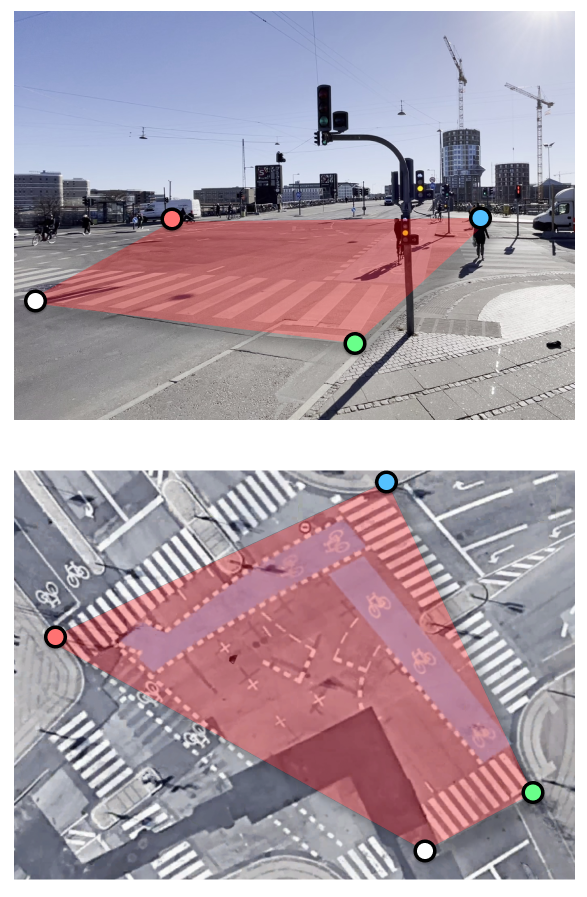
\includegraphics[width=1.0\columnwidth]{projection_figure} 
\end{tabular}
\captionof{figure}{Reference points on map projection}

% To (x, y) coordinates are on the vertical plane of the video. To gain insight into the desire paths of the cyclists we projected the (x, y) coordinate down to the horizontal plane(the street) of the image.
% To do this we used the equation: 
% \begin{equation}
% 	y = y + h ⁄ 2
% \end{equation}

\subsection{Warped perspective}
With the tracks projected onto the roads surface we now warp (x, y) points in order to get a top-down view of the cyclist tracks.
This is achieved by calculating the homography matrix (H) between the source image and the destination image. The homography matrix being a 

\section{Results}

Give the results of your research. Do not, at this stage, try to interpret the results – simply report them. 
This section may include graphs, charts, diagrams etc. (clearly labelled). Be very careful about copyright if you are using published charts, tables, illustrations etc.


\section{Discussion}

Interpret your findings. What do they show? Were they what you expected? 
Could your research have been done in a better way?

\section{Conclusion}

These should follow on logically from the Findings and Discussion sections. Summarize the key points of your findings and show whether they prove or disprove your hypothesis. 
If you have been asked to, you can make recommendations arising from your research.

%----------------------------------------------------------------------------------------
%	BIBLIOGRAPHY
%----------------------------------------------------------------------------------------

\printbibliography[title={Bibliography}] % Print the bibliography, section title in curly brackets


%----------------------------------------------------------------------------------------

\end{document}